			\begin{tikzpicture}	[scale=0.25,rotate=90]	
			\centering
			\onslide<1->{
				\node(image)[scale=0.85,rotate=0] at (-5,-1.5){
					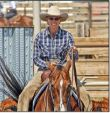
\includegraphics[scale=0.6]{images/cowboy.JPG}
				};

				\node[scale=0.85] at (-5,0-5.8){\tiny{Input}};
			}
				
			\onslide<2->{
					\renewcommand{\forefillColor}{black!50!white}
					\renewcommand{\borderColor}{white}
					\renewcommand{\toprsidefillcolor}{red}
				\node(image)[scale=0.85,rotate=0] at (-5,-1.5){
										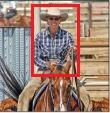
\includegraphics[scale=0.6]{images/cowboy_true.jpg}
									};
					\draw[->,line width=0.25mm](-2,-1.5)--(0,-1.5);
						% Convolution Layer
						\renewcommand{\forefillColor}{red!50!white}
						\renewcommand{\borderColor}{white}
						\renewcommand{\toprsidefillcolor}{red!50!white!50}
						\pgfmathsetmacro{\seedx}{1}
						\pgfmathsetmacro{\seedy}{0}
										
						\foreach \xct/\yct in {1,...,2}
						{
							\pgfmathsetmacro{\xcti}{\seedx+\xct*0.1}
							\pgfmathsetmacro{\ycti}{\seedy}
							\handmadecube{0.5}{4.5}{2.5}{\xcti}{\ycti}
						}
						\node[scale=0.85] at (1+0.5,0-4.8){\tiny{Conv}};
					
									% Pooling Layer
									\renewcommand{\forefillColor}{blue!50!white}
									\renewcommand{\borderColor}{white}
									\renewcommand{\toprsidefillcolor}{blue!50!white!50}
									
									\pgfmathsetmacro{\seedx}{2.5}
									\pgfmathsetmacro{\seedy}{0}
									
									\foreach \xct/\yct in {1}
									{
										%				\pgfmathsetmacro{\xcti}{\seedx+\xct*0.1}
										%				\pgfmathsetmacro{\ycti}{\seedy}
										
										\pgfmathsetmacro{\xcti}{\seedx+\xct*0.1}
										\pgfmathsetmacro{\ycti}{\seedy}
										\handmadecube{0.5}{3.8}{1.8}{\xcti}{\ycti}
									}
									\node[scale=0.85] at (0.5+2.8,0-4.2){\tiny{Max-pool}};
					}
			\onslide<3->{
											
				\foreach \xct in {1,2,3}
				{
					\filldraw[fill=gray!60](3+\xct,-1) circle(2pt) ;
				}
							
				\draw [thin,step=0.7,draw=blue!40!white](6.4,-4.2) grid (12.5,1.4);			
				%\draw [draw=blue!40,thin](6.4,-4.3) grid[step=0.5] (12.5,1.5);
				%\draw [draw=blue!40,thin] (6.4,-4.3) -- (12.5,-4.3);
				\draw [draw=blue!40,thin] (6.4,-4.2) -- (6.4,1.4);
				\draw [draw=blue!40,thin] (12.5,-4.2) -- (12.5,1.4);
			}
		
		\if 0	
		\onslide<4->{			
						
			\pgfmathsetmacro{\x}{10-1}
			\pgfmathsetmacro{\y}{0-1}
						
						\pgfmathsetmacro{\x}{\x-0.5}
						\pgfmathsetmacro{\y}{\y-1.8}
						%\filldraw[fill=red, draw=red,line width=0.5mm] (\x+1.4,\y+0.85) rectangle (\x+1.9,\y+1.35);
						\draw[draw=red,line width=0.4mm] (\x,\y) rectangle (\x+3.5,\y+2.5);		
					}
		\fi		
			\onslide<3->{			
				\pgfmathsetmacro{\x}{10-1}
				\pgfmathsetmacro{\y}{0-1}
									
				\pgfmathsetmacro{\x}{\x-0.5}
				\pgfmathsetmacro{\y}{\y-1.8}
				\filldraw[fill=green, draw=green,line width=0.5mm] (\x+0.7,\y+0.75) rectangle (\x+1.2,\y+1.25);			
			
			%\draw[draw=green,line width=0.7mm] (\x-0.5,\y-0.5) rectangle (\x+2.5,\y+2.5);			
			
			%\node (A1) at (9.5,-3) {};			
			%\node (A3) at (13,-16.1) {};	
			%\path [->,line width=0.3mm] (A3) edge (A1);
							
		}
		\onslide<4->{
			\node(image)[scale=0.85,rotate=0] at (-5,-1.5){
				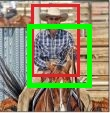
\includegraphics[scale=0.6]{images/cowboy_true_green.jpg}
			};

			\node[scale=0.85] at (-5,0-5.8){\tiny{Input}};
		}
	    \onslide<5->{
   			\node(image)[scale=0.85,rotate=0] at (-5,-1.5){
   				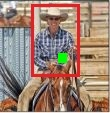
\includegraphics[scale=0.6]{images/cowboy_true_centre.jpg}
   			};
	    
   			\node[scale=0.85] at (-5,0-5.8){\tiny{Input}};
   		}
   		\onslide<7->{
			\colorlet{custom_pink}{pink!50}
			
			\newcommand{\lightercolor}[3]{% Reference Color, Percentage, New Color Name
	    	\colorlet{#3}{#1!#2!white}
			}
			\lightercolor{custom_pink}{30}{LightPink}
	 					
			\filldraw[fill=pink, draw=pink,line width=0.5mm, opacity = 0.7] (-7,-3) rectangle (-3,-1);
  			%\node(image)[scale=0.9,rotate=0] at (-5,-2.2){
  			%	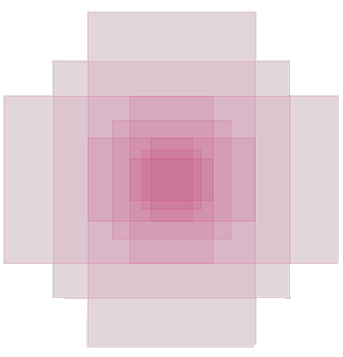
\includegraphics[scale=0.08]{images/achor_boxes_crop.png}
  			%};

  			%\node[scale=0.85] at (-5,0-5.8){\tiny{Input}};
   		}
							
		\onslide<7->{
					\draw (13,-5) grid[xstep=1,ystep=1] (14,3);			
					\node (x1) at (13.5,2.5) {\tiny{$x_1$}};
					\node (x2) at (13.5,1.5) {\tiny{$x_2$}};
					
					\foreach \y in {1,2,...,5}{
						\node (x2) at (13.5,1.5-\y) {\tiny{$\cdot$}};
					}
					
					\node (x2) at (13.5,-4.5) {\tiny{$\cdot$}};
					
					\draw[->](11.8,-1)--(12.8,-1);
					
					\node(A) at (13.5,-1){};
					\node(B)[draw,rounded corners] at (16.5,3){\scriptsize{Classification}};
					\path[draw,line width=0.25mm,->] (A) edge (B);		
					
		}
		\onslide<8->{
			\node(C)[draw,rounded corners] at (16.5,-5){\scriptsize{Regression}};
			\path[draw,line width=0.25mm,->] (A) edge (C);
		}
							
			
			\end{tikzpicture}
			
			\column{0.2\textwidth}
			\begin{tikzpicture}[scale=1]
			\onslide<6->{
						\node(image)[scale=0.55,rotate=0] at (0,0){
										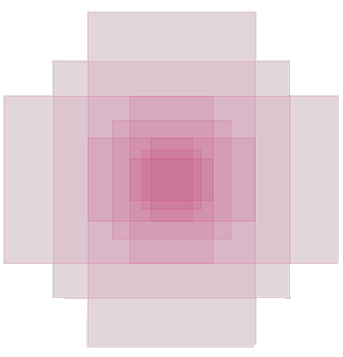
\includegraphics[scale=0.6]{images/achor_boxes_crop.png}
									};
					}
			\end{tikzpicture}
			\if 0
			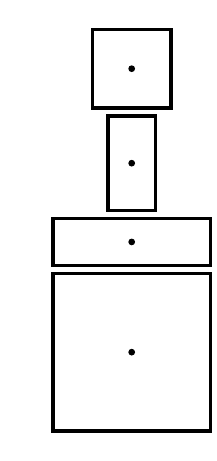
\begin{tikzpicture}[scale=1]
			\hspace*{0.3cm}
			\onslide<3->{
				
				\draw[black, very thick] (0,0)rectangle (2,2);
				\draw[black, very thick] (0,2.1)rectangle (2,2.7);
				\draw[black, very thick] (0.7,2.8)rectangle (1.3,4);
				\draw[black, very thick] (0.5,4.1)rectangle (1.5,5.1);
				
				\filldraw [black] (1,1) circle (1pt);
				\filldraw [black] (1,2.4) circle (1pt);
				\filldraw [black] (1,3.4) circle (1pt);
				\filldraw [black] (1,4.6) circle (1pt);
				
			}
			
			\end{tikzpicture}
			\fi
